\begin{figure}[ht]
  \centering
  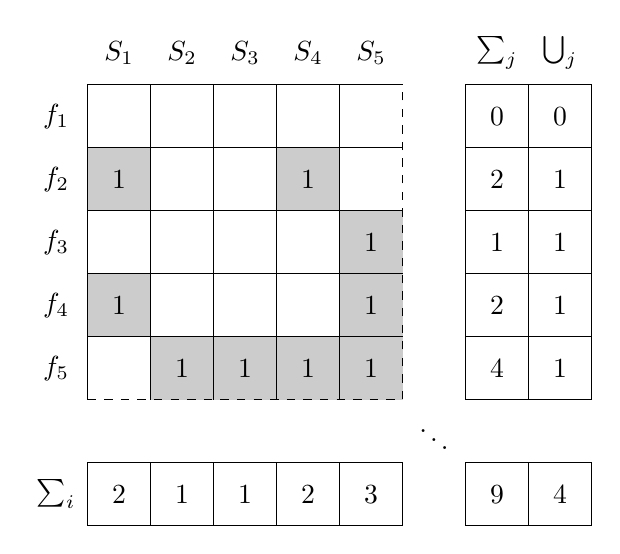
\begin{tikzpicture}[x=8mm, y=8mm]
    % Generated by FA_management/iverson_grid/iverson_grid.py from a markdown table (5 rows, 5 columns).
    % Coordinates: x is horizontal (column j at x = j), y is vertical (row f_i at y = 7 - i, so f_1 is at the top).
    % Grey cells, where f_i belongs to S_j (the Iverson bracket is 1), listed row by row as i/j
    \foreach \row/\col in {%
                          % f_1: none
      2/1, 2/4,           % f_2: S_1, S_4
      3/5,                % f_3: S_5
      4/1, 4/5,           % f_4: S_1, S_5
      5/2, 5/3, 5/4, 5/5  % f_5: S_2, S_3, S_4, S_5
    } {
      \fill[black!20] (\col - 0.5, 6.5 - \row) rectangle ++(1, 1);
      \node at (\col, 7 - \row) {$1$};
    }
    % Headers
    \foreach \col in {1, ..., 5} {\node at (\col, 7) {$S_{\col}$};}
    \node at (7, 7) {$\sum_j$};
    \node at (8, 7) {$\bigcup_j$};
    % Rows f_1, ..., f_5: label, row sum, union bracket
    \foreach \row/\rowsum/\union in {1/0/0, 2/2/1, 3/1/1, 4/2/1, 5/4/1} {
      \node at (0, 7 - \row) {$f_{\row}$};
      \node at (7, 7 - \row) {$\rowsum$};
      \node at (8, 7 - \row) {$\union$};
    }
    % The rows and the columns go on
    \node at (6, 1) {$\ddots$};
    % Row of column sums
    \node at (0, 0) {$\sum_i$};
    \foreach \col/\colsum in {1/2, 2/1, 3/1, 4/2, 5/3} {\node at (\col, 0) {$\colsum$};}
    \node at (7, 0) {$9$};
    \node at (8, 0) {$4$};
    % Inner lines of the 5 x 5 matrix
    \foreach \y in {2.5, 3.5, 4.5, 5.5} {\draw (0.5, \y) -- (5.5, \y);}
    \foreach \x in {1.5, 2.5, 3.5, 4.5} {\draw (\x, 1.5) -- (\x, 6.5);}
    % Lower and right edges of the matrix, dashed
    \draw[dashed] (0.5, 1.5) -- (5.5, 1.5) -- (5.5, 6.5);
    % Upper and left edges of the matrix
    \draw (0.5, 1.5) -- (0.5, 6.5) -- (5.5, 6.5);
    % Framed vectors: the column of row sums, the column of union brackets, the row of column sums, and the totals.
    % Each is a closed box; nothing is drawn between them, around the diagonal dots.
    \draw (6.5, 1.5) rectangle (7.5, 6.5);
    \draw (7.5, 1.5) rectangle (8.5, 6.5);
    \foreach \y in {2.5, 3.5, 4.5, 5.5} {\draw (6.5, \y) -- (8.5, \y);}
    \draw (0.5, -0.5) rectangle (5.5, 0.5);
    \foreach \x in {1.5, 2.5, 3.5, 4.5} {\draw (\x, -0.5) -- (\x, 0.5);}
    \draw (6.5, -0.5) rectangle (8.5, 0.5);
    \draw (7.5, -0.5) -- (7.5, 0.5);
  \end{tikzpicture}
  \caption{The inequality \eqref{1.7:inequality-boolean-series} for the first five terms and five of the $S_j$. A grey
    cell in row $f_i$ and column $S_j$ means $f_i \in S_j$; the dashed edges and the diagonal dots indicate that the
    rows and the columns go on. The left-hand side counts the rows that contain a grey cell (column $\bigcup_j$): $4$.
    The right-hand side counts the grey cells, by rows (column $\sum_j$) or by columns (row $\sum_i$): $9$ either way.
    Each row contributes at most $1$ on the left and its number of grey cells on the right.}
  \label{1.7:figure-Iverson-grid}
\end{figure}
